%% Revised manuscript, SOFTX-D-26-01093 (draft of 2026-10-03).
%%
%% Every measured number is \claim{id} (from reproduce/claims.csv through
%% paper/numbers.tex) or, until the campaign on v2.6.0-rc1 has produced it,
%% \pending{id}. reproduce/lint_numbers.py lists every number typed by hand and
%% every \pending left; the text is done when it reports none.
%%
%% Word budget for the main text (template limit 4000): motivation 550,
%% software description 1350, illustrative examples 1250, impact 600,
%% conclusions 200. Abstract about 100. Six figures at most.
%% Each section names the reviewer points it answers (R1-R11 as numbered in
%% softwarex-revision/response-to-reviewers.md) and the campaign experiment
%% (E1-E9, cluster_bringup/campaign/README.md) its numbers come from.

\documentclass[preprint,12pt,a4paper]{elsarticle}
\usepackage{amssymb}
\usepackage{booktabs}
\usepackage{xcolor}
\newcommand{\hte}{\texttt{hines\_\allowbreak tree\_\allowbreak eliminate}}
\newcommand{\ccm}{\texttt{chip\_\allowbreak channel\_\allowbreak multiloop}}
%% \claim{id}: a value make_numbers.py computed from the raw data; an unknown id
%% stops the build. \pending{id}: a value the campaign has not produced yet.
% generated by reproduce/make_numbers.py from reproduce/claims.csv -- do not edit
% \claim{id} prints a published value; an unknown id stops the build.
\expandafter\def\csname claim@singlecomp_cuda_a40_n500\endcsname{1.5}
\expandafter\def\csname claim@singlecomp_cuda_a40_n500_sd\endcsname{0.1}
\expandafter\def\csname claim@singlecomp_cuda_a40_n5000\endcsname{8.7}
\expandafter\def\csname claim@singlecomp_cuda_a40_n5000_sd\endcsname{0.3}
\expandafter\def\csname claim@singlecomp_cuda_a40_n50000\endcsname{21.0}
\expandafter\def\csname claim@singlecomp_cuda_a40_n50000_sd\endcsname{0.3}
\expandafter\def\csname claim@singlecomp_cuda_a100_n500\endcsname{1.8}
\expandafter\def\csname claim@singlecomp_cuda_a100_n500_sd\endcsname{0.3}
\expandafter\def\csname claim@singlecomp_cuda_a100_n5000\endcsname{9.7}
\expandafter\def\csname claim@singlecomp_cuda_a100_n5000_sd\endcsname{0.4}
\expandafter\def\csname claim@singlecomp_cuda_a100_n50000\endcsname{21.9}
\expandafter\def\csname claim@singlecomp_cuda_a100_n50000_sd\endcsname{0.3}
\expandafter\def\csname claim@singlecomp_ocl_a40_n500\endcsname{1.5}
\expandafter\def\csname claim@singlecomp_ocl_a40_n5000\endcsname{7.5}
\expandafter\def\csname claim@singlecomp_ocl_a40_n50000\endcsname{19.2}
\expandafter\def\csname claim@singlecomp_ocl_a100_n500\endcsname{1.7}
\expandafter\def\csname claim@singlecomp_ocl_a100_n5000\endcsname{8.7}
\expandafter\def\csname claim@singlecomp_ocl_a100_n50000\endcsname{20.4}
\expandafter\def\csname claim@cuda_parity_v\endcsname{7e-08}
\expandafter\def\csname claim@multicomp_step_a40_n100\endcsname{0.2}
\expandafter\def\csname claim@multicomp_step_a40_n100_sd\endcsname{0.21}
\expandafter\def\csname claim@multicomp_e2e_a40_n100\endcsname{0.43}
\expandafter\def\csname claim@multicomp_e2e_a40_n100_sd\endcsname{0.05}
\expandafter\def\csname claim@multicomp_step_a40_n500\endcsname{1.1}
\expandafter\def\csname claim@multicomp_step_a40_n500_sd\endcsname{0.06}
\expandafter\def\csname claim@multicomp_e2e_a40_n500\endcsname{0.77}
\expandafter\def\csname claim@multicomp_e2e_a40_n500_sd\endcsname{0.02}
\expandafter\def\csname claim@multicomp_step_a40_n1000\endcsname{2.0}
\expandafter\def\csname claim@multicomp_step_a40_n1000_sd\endcsname{0.12}
\expandafter\def\csname claim@multicomp_e2e_a40_n1000\endcsname{1.10}
\expandafter\def\csname claim@multicomp_e2e_a40_n1000_sd\endcsname{0.08}
\expandafter\def\csname claim@multicomp_step_a40_n2000\endcsname{4.5}
\expandafter\def\csname claim@multicomp_step_a40_n2000_sd\endcsname{0.54}
\expandafter\def\csname claim@multicomp_e2e_a40_n2000\endcsname{1.37}
\expandafter\def\csname claim@multicomp_e2e_a40_n2000_sd\endcsname{0.06}
\expandafter\def\csname claim@multicomp_step_a40_n3000\endcsname{6.7}
\expandafter\def\csname claim@multicomp_step_a40_n3000_sd\endcsname{0.10}
\expandafter\def\csname claim@multicomp_e2e_a40_n3000\endcsname{1.87}
\expandafter\def\csname claim@multicomp_e2e_a40_n3000_sd\endcsname{0.08}
\expandafter\def\csname claim@multicomp_step_a40_n5000\endcsname{6.9}
\expandafter\def\csname claim@multicomp_step_a40_n5000_sd\endcsname{0.18}
\expandafter\def\csname claim@multicomp_e2e_a40_n5000\endcsname{2.60}
\expandafter\def\csname claim@multicomp_e2e_a40_n5000_sd\endcsname{0.06}
\expandafter\def\csname claim@multicomp_step_a40_n7000\endcsname{9.8}
\expandafter\def\csname claim@multicomp_step_a40_n7000_sd\endcsname{0.24}
\expandafter\def\csname claim@multicomp_e2e_a40_n7000\endcsname{2.92}
\expandafter\def\csname claim@multicomp_e2e_a40_n7000_sd\endcsname{0.05}
\expandafter\def\csname claim@multicomp_step_a40_n10000\endcsname{13.7}
\expandafter\def\csname claim@multicomp_step_a40_n10000_sd\endcsname{0.22}
\expandafter\def\csname claim@multicomp_e2e_a40_n10000\endcsname{3.01}
\expandafter\def\csname claim@multicomp_e2e_a40_n10000_sd\endcsname{0.04}
\expandafter\def\csname claim@multicomp_step_a40_n15000\endcsname{20.3}
\expandafter\def\csname claim@multicomp_step_a40_n15000_sd\endcsname{0.23}
\expandafter\def\csname claim@multicomp_e2e_a40_n15000\endcsname{3.27}
\expandafter\def\csname claim@multicomp_e2e_a40_n15000_sd\endcsname{0.05}
\expandafter\def\csname claim@multicomp_step_a40_n20000\endcsname{25.3}
\expandafter\def\csname claim@multicomp_step_a40_n20000_sd\endcsname{0.39}
\expandafter\def\csname claim@multicomp_e2e_a40_n20000\endcsname{3.39}
\expandafter\def\csname claim@multicomp_e2e_a40_n20000_sd\endcsname{0.04}
\expandafter\def\csname claim@multicomp_step_a40_n30000\endcsname{31.9}
\expandafter\def\csname claim@multicomp_step_a40_n30000_sd\endcsname{0.46}
\expandafter\def\csname claim@multicomp_e2e_a40_n30000\endcsname{3.53}
\expandafter\def\csname claim@multicomp_e2e_a40_n30000_sd\endcsname{0.05}
\expandafter\def\csname claim@multicomp_step_a40_n40000\endcsname{35.2}
\expandafter\def\csname claim@multicomp_step_a40_n40000_sd\endcsname{0.44}
\expandafter\def\csname claim@multicomp_e2e_a40_n40000\endcsname{3.56}
\expandafter\def\csname claim@multicomp_e2e_a40_n40000_sd\endcsname{0.05}
\expandafter\def\csname claim@multicomp_step_a40_n50000\endcsname{37.3}
\expandafter\def\csname claim@multicomp_step_a40_n50000_sd\endcsname{0.31}
\expandafter\def\csname claim@multicomp_e2e_a40_n50000\endcsname{3.62}
\expandafter\def\csname claim@multicomp_e2e_a40_n50000_sd\endcsname{0.05}
\expandafter\def\csname claim@multicomp_step_a100_n100\endcsname{0.3}
\expandafter\def\csname claim@multicomp_step_a100_n100_sd\endcsname{0.02}
\expandafter\def\csname claim@multicomp_e2e_a100_n100\endcsname{0.61}
\expandafter\def\csname claim@multicomp_e2e_a100_n100_sd\endcsname{0.02}
\expandafter\def\csname claim@multicomp_step_a100_n500\endcsname{1.7}
\expandafter\def\csname claim@multicomp_step_a100_n500_sd\endcsname{0.12}
\expandafter\def\csname claim@multicomp_e2e_a100_n500\endcsname{1.04}
\expandafter\def\csname claim@multicomp_e2e_a100_n500_sd\endcsname{0.03}
\expandafter\def\csname claim@multicomp_step_a100_n1000\endcsname{3.1}
\expandafter\def\csname claim@multicomp_step_a100_n1000_sd\endcsname{0.17}
\expandafter\def\csname claim@multicomp_e2e_a100_n1000\endcsname{1.46}
\expandafter\def\csname claim@multicomp_e2e_a100_n1000_sd\endcsname{0.05}
\expandafter\def\csname claim@multicomp_step_a100_n2000\endcsname{6.4}
\expandafter\def\csname claim@multicomp_step_a100_n2000_sd\endcsname{0.29}
\expandafter\def\csname claim@multicomp_e2e_a100_n2000\endcsname{1.57}
\expandafter\def\csname claim@multicomp_e2e_a100_n2000_sd\endcsname{0.05}
\expandafter\def\csname claim@multicomp_step_a100_n3000\endcsname{12.0}
\expandafter\def\csname claim@multicomp_step_a100_n3000_sd\endcsname{0.51}
\expandafter\def\csname claim@multicomp_e2e_a100_n3000\endcsname{1.89}
\expandafter\def\csname claim@multicomp_e2e_a100_n3000_sd\endcsname{0.04}
\expandafter\def\csname claim@multicomp_step_a100_n5000\endcsname{14.5}
\expandafter\def\csname claim@multicomp_step_a100_n5000_sd\endcsname{0.51}
\expandafter\def\csname claim@multicomp_e2e_a100_n5000\endcsname{2.66}
\expandafter\def\csname claim@multicomp_e2e_a100_n5000_sd\endcsname{0.03}
\expandafter\def\csname claim@multicomp_step_a100_n7000\endcsname{22.0}
\expandafter\def\csname claim@multicomp_step_a100_n7000_sd\endcsname{0.52}
\expandafter\def\csname claim@multicomp_e2e_a100_n7000\endcsname{3.08}
\expandafter\def\csname claim@multicomp_e2e_a100_n7000_sd\endcsname{0.03}
\expandafter\def\csname claim@multicomp_step_a100_n10000\endcsname{30.5}
\expandafter\def\csname claim@multicomp_step_a100_n10000_sd\endcsname{0.83}
\expandafter\def\csname claim@multicomp_e2e_a100_n10000\endcsname{3.23}
\expandafter\def\csname claim@multicomp_e2e_a100_n10000_sd\endcsname{0.04}
\expandafter\def\csname claim@multicomp_step_a100_n15000\endcsname{42.3}
\expandafter\def\csname claim@multicomp_step_a100_n15000_sd\endcsname{0.91}
\expandafter\def\csname claim@multicomp_e2e_a100_n15000\endcsname{3.52}
\expandafter\def\csname claim@multicomp_e2e_a100_n15000_sd\endcsname{0.03}
\expandafter\def\csname claim@multicomp_step_a100_n20000\endcsname{51.6}
\expandafter\def\csname claim@multicomp_step_a100_n20000_sd\endcsname{1.33}
\expandafter\def\csname claim@multicomp_e2e_a100_n20000\endcsname{3.71}
\expandafter\def\csname claim@multicomp_e2e_a100_n20000_sd\endcsname{0.04}
\expandafter\def\csname claim@multicomp_step_a100_n30000\endcsname{66.1}
\expandafter\def\csname claim@multicomp_step_a100_n30000_sd\endcsname{1.45}
\expandafter\def\csname claim@multicomp_e2e_a100_n30000\endcsname{3.87}
\expandafter\def\csname claim@multicomp_e2e_a100_n30000_sd\endcsname{0.05}
\expandafter\def\csname claim@multicomp_step_a100_n40000\endcsname{75.5}
\expandafter\def\csname claim@multicomp_step_a100_n40000_sd\endcsname{1.31}
\expandafter\def\csname claim@multicomp_e2e_a100_n40000\endcsname{3.90}
\expandafter\def\csname claim@multicomp_e2e_a100_n40000_sd\endcsname{0.04}
\expandafter\def\csname claim@multicomp_step_a100_n50000\endcsname{80.8}
\expandafter\def\csname claim@multicomp_step_a100_n50000_sd\endcsname{1.31}
\expandafter\def\csname claim@multicomp_e2e_a100_n50000\endcsname{3.90}
\expandafter\def\csname claim@multicomp_e2e_a100_n50000_sd\endcsname{0.07}
\expandafter\def\csname claim@ksweep_cpu_k200\endcsname{5.86}
\expandafter\def\csname claim@ksweep_gpu_k200\endcsname{1.37}
\expandafter\def\csname claim@ksweep_e2e_k200\endcsname{4.28}
\expandafter\def\csname claim@ksweep_e2e_k200_sd\endcsname{0.14}
\expandafter\def\csname claim@ksweep_cpu_k500\endcsname{13.00}
\expandafter\def\csname claim@ksweep_gpu_k500\endcsname{1.42}
\expandafter\def\csname claim@ksweep_e2e_k500\endcsname{9.18}
\expandafter\def\csname claim@ksweep_e2e_k500_sd\endcsname{0.28}
\expandafter\def\csname claim@ksweep_cpu_k1000\endcsname{24.87}
\expandafter\def\csname claim@ksweep_gpu_k1000\endcsname{1.49}
\expandafter\def\csname claim@ksweep_e2e_k1000\endcsname{16.73}
\expandafter\def\csname claim@ksweep_e2e_k1000_sd\endcsname{0.40}
\expandafter\def\csname claim@ksweep_cpu_k2000\endcsname{48.03}
\expandafter\def\csname claim@ksweep_gpu_k2000\endcsname{1.63}
\expandafter\def\csname claim@ksweep_e2e_k2000\endcsname{29.48}
\expandafter\def\csname claim@ksweep_e2e_k2000_sd\endcsname{1.02}
\expandafter\def\csname claim@ksweep_cpu_k5000\endcsname{116.75}
\expandafter\def\csname claim@ksweep_gpu_k5000\endcsname{2.05}
\expandafter\def\csname claim@ksweep_e2e_k5000\endcsname{57.01}
\expandafter\def\csname claim@ksweep_e2e_k5000_sd\endcsname{0.98}
\expandafter\def\csname claim@ksweep_e2e_k5000_recheck\endcsname{55.4}
\expandafter\def\csname claim@ksweep_e2e_k5000_recheck_sd\endcsname{1.6}
\expandafter\def\csname claim@ksweep_fixed_cpu\endcsname{1.6}
\expandafter\def\csname claim@ksweep_perstep_cpu\endcsname{2.31e-02}
\expandafter\def\csname claim@ksweep_fixed_gpu\endcsname{1.3}
\expandafter\def\csname claim@ksweep_perstep_gpu\endcsname{1.41e-04}
\expandafter\def\csname claim@ksweep_perstep_ratio\endcsname{164}
\expandafter\def\csname claim@construction_exponent_before\endcsname{2.31}
\expandafter\def\csname claim@construction_exponent_after\endcsname{0.99}
\expandafter\def\csname claim@construction_527k_s\endcsname{14.6}
\expandafter\def\csname claim@construction_527k_s_sd\endcsname{0.2}
\expandafter\def\csname claim@construction_1700k_s\endcsname{51.5}
\expandafter\def\csname claim@construction_1700k_s_sd\endcsname{0.6}
\expandafter\def\csname claim@pgenesis_t1\endcsname{2.39}
\expandafter\def\csname claim@pgenesis_t2\endcsname{1.26}
\expandafter\def\csname claim@pgenesis_t4\endcsname{0.76}
\expandafter\def\csname claim@pgenesis_t8\endcsname{0.59}
\expandafter\def\csname claim@pgenesis_eff_p2\endcsname{0.95}
\expandafter\def\csname claim@pgenesis_speedup_p4\endcsname{3.1}
\expandafter\def\csname claim@pgenesis_speedup_p8\endcsname{4.0}
\expandafter\def\csname claim@vanet2_genesis_published_s\endcsname{46.9}
\expandafter\def\csname claim@vanet2_genesis_published_s_sd\endcsname{2.1}
\expandafter\def\csname claim@vanet2_genesis_1solver_s\endcsname{33.2}
\expandafter\def\csname claim@vanet2_genesis_1solver_s_sd\endcsname{0.7}
\expandafter\def\csname claim@vanet2_coreneuron_cpu_s\endcsname{76.5}
\expandafter\def\csname claim@vanet2_neuron_cpu_s\endcsname{95.8}
\expandafter\def\csname claim@vanet2_neuron_channelbuilder_s\endcsname{123.3}
\expandafter\def\csname claim@vanet2_arbor_a100_s\endcsname{149.4}
\expandafter\def\csname claim@vanet2_coreneuron_a100_s\endcsname{27.0}
\expandafter\def\csname claim@vanet2_cpu_1solver_s\endcsname{34.9}
\expandafter\def\csname claim@vanet2_gpu_1solver_s\endcsname{36.3}
\expandafter\def\csname claim@vanet2_cpu_published_20aug_s\endcsname{48.9}
\expandafter\def\csname claim@vanet2_gpu_over_cpu\endcsname{1.04}
\expandafter\def\csname claim@vanet2_vs_coreneuron_cpu\endcsname{2.30}
\expandafter\def\csname claim@vanet2_vs_neuron_cpu\endcsname{2.89}
\expandafter\def\csname claim@vanet2_coreneuron_over_neuron\endcsname{1.25}
\expandafter\def\csname claim@vanet2_coreneuron_gpu_ahead\endcsname{1.23}
\expandafter\def\csname claim@vanet2_coreneuron_gpu_over_own_cpu\endcsname{2.83}
\expandafter\def\csname claim@vanet2_1solver_speedup\endcsname{1.41}
\expandafter\def\csname claim@vanet2_spikes_coreneuron_a100\endcsname{592\,865}
\expandafter\def\csname claim@vanet2_spikes_genesis_cpu\endcsname{545\,371}
\expandafter\def\csname claim@vanet2_spikes_genesis_gpu\endcsname{551\,117}
\expandafter\def\csname claim@vanet2_spike_agreement_pct\endcsname{1.1}
\expandafter\def\csname claim@mccross_arbor_cpu_k5000\endcsname{1.09}
\expandafter\def\csname claim@mccross_arbor_cpu_k5000_sd\endcsname{0.04}
\expandafter\def\csname claim@mccross_coreneuron_cpu_k5000\endcsname{60.94}
\expandafter\def\csname claim@mccross_coreneuron_cpu_k5000_sd\endcsname{0.15}
\expandafter\def\csname claim@mccross_neuron_cpu_k5000\endcsname{82.82}
\expandafter\def\csname claim@mccross_neuron_cpu_k5000_sd\endcsname{1.99}
\expandafter\def\csname claim@mccross_genesis_cpu_k5000\endcsname{123.41}
\expandafter\def\csname claim@mccross_genesis_cpu_k5000_sd\endcsname{1.73}
\expandafter\def\csname claim@mccross_genesis_over_coreneuron_cpu\endcsname{2.03}
\expandafter\def\csname claim@crossover_genesis_a100_k5000\endcsname{1.59}
\expandafter\def\csname claim@crossover_genesis_a100_k5000_sd\endcsname{0.01}
\expandafter\def\csname claim@crossover_genesis_a100_k50000\endcsname{4.56}
\expandafter\def\csname claim@crossover_genesis_a100_k50000_sd\endcsname{0.01}
\expandafter\def\csname claim@crossover_fixed_genesis_a100\endcsname{1.28}
\expandafter\def\csname claim@crossover_perstep_genesis_a100\endcsname{6.564e-05}
\expandafter\def\csname claim@crossover_arbor_a100_k5000\endcsname{1.56}
\expandafter\def\csname claim@crossover_arbor_a100_k5000_sd\endcsname{0.03}
\expandafter\def\csname claim@crossover_arbor_a100_k50000\endcsname{5.95}
\expandafter\def\csname claim@crossover_arbor_a100_k50000_sd\endcsname{0.02}
\expandafter\def\csname claim@crossover_fixed_arbor_a100\endcsname{1.08}
\expandafter\def\csname claim@crossover_perstep_arbor_a100\endcsname{9.733e-05}
\expandafter\def\csname claim@crossover_k_a100\endcsname{6365}
\expandafter\def\csname claim@crossover_ms_a100\endcsname{64}
\expandafter\def\csname claim@crossover_marginal_lower_pct_a100\endcsname{33}
\expandafter\def\csname claim@crossover_arbor_ahead_s_a100\endcsname{0.20}
\expandafter\def\csname claim@crossover_genesis_a40_k5000\endcsname{2.02}
\expandafter\def\csname claim@crossover_genesis_a40_k5000_sd\endcsname{0.01}
\expandafter\def\csname claim@crossover_genesis_a40_k50000\endcsname{8.34}
\expandafter\def\csname claim@crossover_genesis_a40_k50000_sd\endcsname{0.04}
\expandafter\def\csname claim@crossover_fixed_genesis_a40\endcsname{1.35}
\expandafter\def\csname claim@crossover_perstep_genesis_a40\endcsname{1.400e-04}
\expandafter\def\csname claim@crossover_arbor_a40_k5000\endcsname{2.49}
\expandafter\def\csname claim@crossover_arbor_a40_k5000_sd\endcsname{0.01}
\expandafter\def\csname claim@crossover_arbor_a40_k50000\endcsname{15.04}
\expandafter\def\csname claim@crossover_arbor_a40_k50000_sd\endcsname{0.01}
\expandafter\def\csname claim@crossover_fixed_arbor_a40\endcsname{1.10}
\expandafter\def\csname claim@crossover_perstep_arbor_a40\endcsname{2.789e-04}
\expandafter\def\csname claim@crossover_k_a40\endcsname{1811}
\expandafter\def\csname claim@crossover_ms_a40\endcsname{18}
\expandafter\def\csname claim@crossover_marginal_lower_pct_a40\endcsname{50}
\expandafter\def\csname claim@crossover_arbor_ahead_s_a40\endcsname{0.25}
\expandafter\def\csname claim@rate_insensitivity_genesis_gpu\endcsname{0.984}
\expandafter\def\csname claim@rate_insensitivity_arbor_gpu\endcsname{0.999}
\expandafter\def\csname claim@vm_ap_peak_neuron_arbor_mv\endcsname{0.02}
\expandafter\def\csname claim@vm_ap_peak_genesis_lower_mv\endcsname{4.6}
\expandafter\def\csname claim@spiking_accelerable_fraction_pct\endcsname{59}
\expandafter\def\csname claim@fp32_single_ap_v\endcsname{2e-07}
\expandafter\def\csname claim@single_morphology_slower_x\endcsname{20}
\expandafter\def\csname claim@multicomp_build_n50000_s\endcsname{23.8}
\expandafter\def\csname claim@ksweep_step_k5000\endcsname{116.2}
\expandafter\def\csname claim@ocl_trails_cuda_pct_a40\endcsname{8}
\expandafter\def\csname claim@ocl_trails_cuda_pct_a100\endcsname{7}
\expandafter\def\csname claim@multicomp_gpu_phase_a40_s\endcsname{7.83}
\expandafter\def\csname claim@multicomp_gpu_phase_a100_s\endcsname{8.06}
\expandafter\def\csname claim@crossover_setup_overhead_s\endcsname{0.21}
\expandafter\def\csname claim@vanet2_rate_hz\endcsname{27}
\expandafter\def\csname claim@vanet2_rate_min_hz\endcsname{26.8}
\expandafter\def\csname claim@vanet2_rate_max_hz\endcsname{30.1}
\expandafter\def\csname claim@vanet2_spikes_genesis_published\endcsname{536\,600}
\expandafter\def\csname claim@vanet2_spikes_coreneuron_cpu\endcsname{558\,824}
\expandafter\def\csname claim@vanet2_spikes_neuron_channelbuilder\endcsname{574\,138}
\expandafter\def\csname claim@vanet2_spikes_arbor_a100\endcsname{602\,720}
\expandafter\def\csname claim@vanet2_level_at_12500_ratio\endcsname{1.00}
\expandafter\def\csname claim@spiking_speedup_ceiling\endcsname{2.4}
\expandafter\def\csname claim@harness_fix_walltime_change_pct\endcsname{1.3}
\expandafter\def\csname claim@igpu_tree_limit_compartments\endcsname{22\,000}
\providecommand{\claim}[1]{\ifcsname claim@#1\endcsname\csname claim@#1\endcsname\else\errmessage{claim #1 undefined}\fi}

\newcommand{\pending}[1]{\textcolor{red}{\textbf{[\detokenize{#1}]}}}
\usepackage{hyperref}
\setlength{\parindent}{0pt}

\begin{document}

\begin{frontmatter}

%% Title: keep, or name the release (v2.6.0)? Karol to decide.
\title{GENESIS 2.5: optimisation and opt-in OpenCL/CUDA acceleration for the GENESIS/PGENESIS compartmental neural simulator}

\author[1]{Karol Chlasta\corref{cor1}}
\ead{karol@chlasta.pl}
\author[2]{Grzegorz Marcin W\'ojcik}
\ead{gmwojcik@umcs.edu.pl}
\address[1]{Kozminski University, ul. Jagiello\'nska 57/59, 03-301 Warsaw, Poland; WarsawIQ, Al. Jana Paw\l{}a II 43A/37B, 01-001 Warsaw, Poland}
\address[2]{Maria Curie-Sk{\l}odowska University, ul. Akademicka 9, 20-033 Lublin, Poland}
\cortext[cor1]{Corresponding author.}

\begin{abstract}
%% about 100 words (R10). One speed number, one correctness number, one limit.
GENESIS is a long-established compartmental neural simulator. GENESIS~2.5 adds
optional CUDA and OpenCL backends to its \texttt{hsolve} solver, including a GPU
Hines elimination for populations of dendritic trees, without changes to existing
models, scripts or MPI workflows. On a population of 160\,000 compartments the
accelerator runs \pending{e2_max_e2e_a100}$\times$ faster end to end than the CPU
solver; in double precision it reproduces the CPU solver to every printed digit.
Spiking networks that exchange spikes every step gain nothing on the GPU, and we
say why. The release also makes model construction linear and fixes three defects
in the Hines solver of GENESIS~2.4.
\end{abstract}

\begin{keyword}
GENESIS \sep PGENESIS \sep compartmental neural simulation \sep Hines solver \sep GPU \sep CUDA \sep OpenCL
\end{keyword}

\end{frontmatter}

\section*{Required Metadata}
\section*{Current code version}

\begin{table}[!h]
\begin{tabular}{|l|p{6.0cm}|p{6.0cm}|}
\hline
\textbf{Nr.} & \textbf{Code metadata description} & \textbf{Please fill in this column} \\
\hline
C1 & Current code version & v2.6.0 \\
\hline
C2 & Permanent GitHub link to code/repository used for this code version & \url{https://github.com/WarsawIQ/genesis-2.5} (release v2.6.0, archived at \pending{zenodo_doi_v260}) \\
\hline
C3 & Legal Code License & GNU General Public License v2 or later (program); GNU Lesser General Public License v2.1 or later (library portions); see \texttt{LICENSE} \\
\hline
C4 & Code versioning system used & git \\
\hline
C5 & Software code languages, tools, and services used & C, CUDA C++, OpenCL C, MPI (PGENESIS), Python and POSIX shell (reproduction and analysis) \\
\hline
C6 & Compilation requirements, operating environments \& dependencies & Linux x86\_64 or aarch64, GCC, GNU make, flex, bison, ncurses. Optional: CUDA 12.x (tested 12.8 on NVIDIA A40 and A100), an OpenCL 1.2 runtime (tested NVIDIA, AMD ROCm 6.3.1, Mesa rusticl 26.1), MPICH or Open~MPI for PGENESIS \\
\hline
C7 & If available Link to developer documentation/manual & \texttt{README.md}, \path{reproduce/README.md}, \path{paper/docs/REPLICATION.md} \\
\hline
C8 & Support email for questions & karol@chlasta.pl \\
\hline
\end{tabular}
\caption{Code metadata (mandatory)}
\end{table}

\textbf{Main text}\\
\begin{enumerate}

%% ===================================================================== 1
\item Motivation and significance
%% 550 words. R1 (relationship to GENESIS 2.4) goes here.

GENESIS~\cite{bower1998} and its MPI version PGENESIS are among the
longest-maintained compartmental simulators. Models are written as SLI scripts,
cell files and channel prototypes, often accumulated over many years, and the
compute engine is \texttt{hsolve}, an implicit Hines solver~\cite{hines1984efficient}
that compiles a model into a flat program at setup. Until this release every step of
that program ran on the CPU.

\textbf{Relationship to GENESIS~2.4.} %% R1
GENESIS~2.5 is an independently maintained derivative of GENESIS~2.4, released under
the same licence as a fork of the project's repository (\texttt{genesis-sim/genesis-2.4},
last changed in 2019). It is not an official release of the GENESIS project. The second
author has used GENESIS and PGENESIS since his doctoral work and met its maintainer,
Dave Beeman, at the EU Advanced Course in Computational Neuroscience in 2001; the first
author completed his PhD under the second author's supervision. On 30 September 2026
we offered the work to the original project: the solver fixes as a pull request, and
the whole release as its next version. \pending{upstream_status}
%% Outcome by submission: reply / PR number / no reply.

\textbf{Alternatives, and what they ask of a user.} NEURON~\cite{hines1997neuron} with
its engine CoreNEURON~\cite{kumbhar2019coreneuron} and Arbor~\cite{arbor2019} run
compartmental models on GPUs and are strong choices for a new model. For an existing
GENESIS model each means re-expressing it in another description, and establishing
that the port computes the same thing is itself experimental work: for the published
network used below it took a transcription of the channels and a check of spike trains
(Section~3). NEST~\cite{gewaltig2007nest} and Brian~2~\cite{stimberg2019brian} simulate
point neurons. GENESIS~2.5 offers acceleration without migration: the same scripts on
the hardware the user has.

\textbf{Contributions.}
\begin{enumerate}
\item CUDA and OpenCL backends for \texttt{hsolve}, selected at run time, in single or
      double precision, falling back to the CPU for anything they cannot compute.
\item \hte{}, a GPU Hines elimination for populations of dendritic trees.
\item Three fixes to the Hines solver of GENESIS~2.4 and linear model construction,
      which apply with or without a GPU.
\item A comparison with NEURON, CoreNEURON and Arbor in which every arm is measured in
      one session, and a reproduction package that regenerates every number in this
      paper from raw data (Section~3.4).
\end{enumerate}

%% ===================================================================== 2
\item Software description
%% 1350 words. R2 (design decisions, architecture figure), R4 (precision),
%% R6 (execution model), R7 (portability).

\begin{enumerate}
\item Software architecture

%% Fig. 1: architecture diagram (new; replaces the fp32/fp64 divergence figure).
\begin{figure}[!h]
\centering
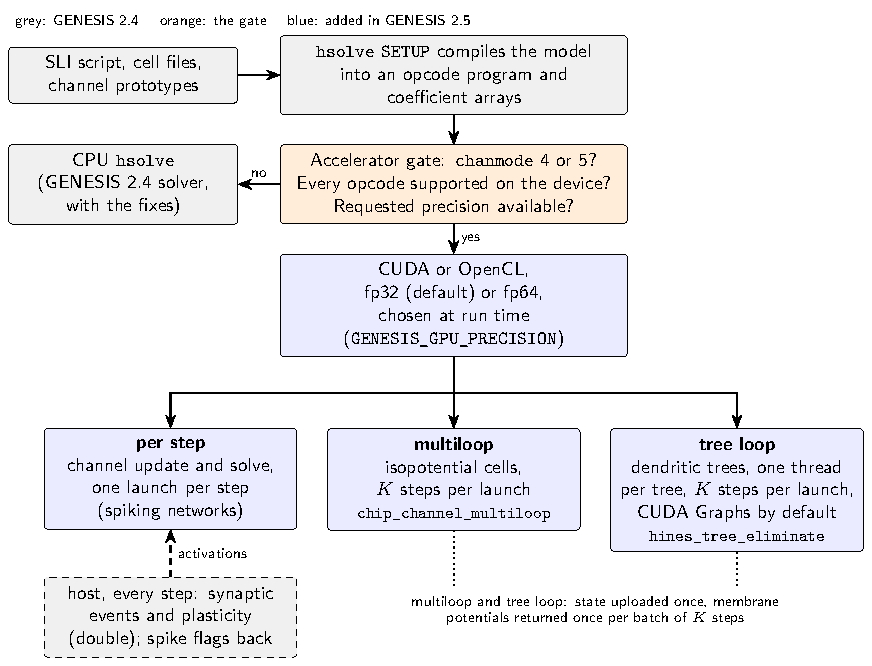
\includegraphics[width=\textwidth]{figures/fig_architecture.pdf}
\caption{How a model reaches the GPU. \texttt{hsolve} compiles the model into an opcode
program at \texttt{SETUP}. A gate checks the program against what the kernels
implement; anything else stays on the CPU. Accepted models run as one of three
dispatches: per step, batched over many steps for isopotential cells
(\ccm{}), or batched for dendritic trees (\hte{}). Synaptic events are delivered by the
host every step.}
\label{fig:architecture}
\end{figure}

The backends sit behind one entry point in \texttt{hsolve}
(Fig.~\ref{fig:architecture}). A user selects them with \texttt{chanmode} and
environment variables; nothing in a model script changes. [Short description of the
three dispatch paths and of what stays on the host.]

\item Design decisions %% R2
\begin{enumerate}
\item \emph{The kernels interpret the solver's own program.} Both backends execute the
      opcode program \texttt{hsolve} already builds, so every model it accepts runs
      unchanged. GPU-native simulators generate code per mechanism instead; interpreting
      costs divergence and a fixed setup time (Section~3), and is what removes the
      migration.
\item \emph{The tree solve needs no synchronisation.} The elimination program of a
      population is block-diagonal: each tree touches only its own rows. One thread per
      tree runs the CPU's elimination with no barrier, once the opcode that joins two
      trees in the CPU program is split per tree.
\item \emph{What the kernels cannot compute is refused, not approximated.} The first
      release accepted models with synaptic, spike, GHK and concentration elements and
      returned plausible wrong voltages. Such programs are now detected at
      \texttt{SETUP} and computed on the CPU.
\item \emph{The device owns the state it computes.} With synaptic input the host
      writes only the slots it owns each step; uploading the whole state, as the first
      release did, overwrote gating variables the kernel had just updated.
\end{enumerate}

\item Precision %% R4
Single precision is the default; \texttt{GENESIS\_GPU\_PRECISION=fp64} selects double
precision at run time in the same binary, and a device without it refuses with a
message and computes on the CPU. In fp64 the GPU reproduces the CPU solver to every
printed digit on our verification models; in fp32 it agrees to
\pending{fp32_single_ap_v}\,V over one action potential. Synaptic weights and
plasticity are computed by the synapse objects on the host in double precision in every
mode; only the resulting activation reaches the device. [Cost of fp64 per card (E2, E4)
and the 10\,s run (E5) are in Section~3.]

\item Execution model %% R6
[One thread per tree: the slowest tree in a warp sets its time
(E7: mixed trees \pending{e7_inter_over_uniform}$\times$ slower than uniform trees of the
same total). Divergence: compartments with different channel sets follow different
opcode streams. Transfers: state goes to the device once and returns once per batch of
$K$ steps. Launch overhead: about \pending{f2_host_us_per_step}\,µs of host time per step against about \pending{f2_kernel_us_per_step}\,µs of
kernel time in the tree loop; CUDA Graphs, on by default for the tree loop since they
change no result, recover \pending{e8_gain_tree_k5000_a100}\% on the A100 and
\pending{e8_gain_tree_k5000_a40}\% on the A40 (E8). The spiking network gains nothing
from graphs (\pending{e8_gain_spiking_a100}\%): its cost is the host's spike delivery
and the synchronisation it forces every step.]

\item Portability %% R7
[OpenCL on NVIDIA A40/A100 and on an AMD Radeon 890M under ROCm and Mesa rusticl (E9):
correctness on all, fp64 under ROCm only, the integrated GPU's size cap and what happens
above it.]
\end{enumerate}

%% ===================================================================== 3
\item Illustrative examples
%% 1250 words. R3, R5, R8, R9; all numbers from the campaign on v2.6.0-rc1.
Every number in this section was measured on release v2.6.0 on the UMCS ``Lunar''
cluster (inf02: Xeon Gold 6342 and NVIDIA A40; inf03: Xeon Platinum 8358 and NVIDIA
A100), CPU arms single-threaded, wall clock around the whole process, means of
replicates run in interleaved order, with uncertainties given as the ratio of means
with the relative sample standard deviations combined in quadrature.

\begin{enumerate}
\item Speed on populations of cells
%% E3 (Table 1: single compartment; Fig. 2: dendritic trees), E2 (Fig. 3: run length).
[Single-compartment network: Table~\ref{tab:single}. Dendritic trees:
Fig.~\ref{fig:trees}, end to end and step phase. Run length: Fig.~\ref{fig:runlength};
the largest end-to-end speedup is \pending{e2_max_e2e_a40}$\times$ on the A40 and
\pending{e2_max_e2e_a100}$\times$ on the A100 (R8), and fp64 costs
\pending{e2_fp64_cost_a40}$\times$ and \pending{e2_fp64_cost_a100}$\times$ the fp32
time.]

\begin{table}[!h]
\centering\small
\pending{tab_single}
\caption{Single-compartment network, $K=50\,000$ steps: speedup of each backend over
the CPU solver (E3, 10 replicates).}
\label{tab:single}
\end{table}

\begin{figure}[!h]
\centering
\pending{fig_trees}
\caption{Dendritic trees, $N\times16$ compartments, 200 steps: speedup over the CPU
solver, end to end and step phase, on the A40 and A100 (E3).}
\label{fig:trees}
\end{figure}

\begin{figure}[!h]
\centering
\pending{fig_runlength}
\caption{End-to-end speedup against run length, $10\,000\times16$ compartments, fp32
and fp64, both cards (E2).}
\label{fig:runlength}
\end{figure}

\item Against other simulators %% R3, R9
%% E1 (Table: spiking network, one session), E4 (Fig. 4: crossover with Arbor,
%% fp32 and fp64), E6 (profiles: why the ranking differs).
[Spiking network (Table~\ref{tab:sim}, one session on inf03, 5 replicates). Dendritic
trees against Arbor on the GPU (Fig.~\ref{fig:crossover}): crossover at
\pending{e4_crossover_ms_a100}\,ms in fp32 and \pending{e4_crossover_ms_fp64_a100}\,ms
when GENESIS also computes in double. Why the order differs between the workloads, from
CPU profiles (E6): channel update, linear solve and event delivery take
\pending{e6_shares_genesis_spk} of GENESIS's time and \pending{e6_shares_cn_spk} of
CoreNEURON's on the network, \pending{e6_shares_genesis_tree} and
\pending{e6_shares_cn_tree} on the trees.]

\begin{table}[!h]
\centering\small
\pending{tab_sim}
\caption{Vogels--Abbott COBAHH network~\cite{vogels2005signal,brette2007simulation},
4000 cells, 5\,s: wall time of every arm in one session on inf03 (E1, 5 replicates,
interleaved).}
\label{tab:sim}
\end{table}

\begin{figure}[!h]
\centering
\pending{fig_crossover}
\caption{GENESIS and Arbor on the same GPU against run length, GENESIS in fp32 and fp64
(E4).}
\label{fig:crossover}
\end{figure}

\item When to use the GPU %% R5
\begin{table}[!h]
\centering\small
\begin{tabular}{p{4cm}p{2.6cm}p{6.2cm}}
\toprule
Workload & GPU? & Why \\
\midrule
One detailed morphology & No & one thread per tree; the GPU is slower than the CPU \\
Population of dendritic trees & Yes, from about \pending{regime_trees_min_n} cells & many trees fill the device (Fig.~\ref{fig:trees}) \\
Isopotential cells without synapses & Yes & \pending{regime_single_max}$\times$ at $N=50\,000$ (Table~\ref{tab:single}) \\
Spiking network, zero axonal delay & No gain & spikes are exchanged every step, so every step is a dispatch (Table~\ref{tab:sim}) \\
Long runs & Gain grows with length & the fixed setup cost is amortised (Fig.~\ref{fig:runlength}) \\
\bottomrule
\end{tabular}
\caption{Where acceleration helps.}
\label{tab:regimes}
\end{table}

\item Correctness over a long run %% R4
%% E5, Fig. 6 (or a table if the figure budget is short).
[10\,s of the network in fp32, fp64 and on the CPU: spike counts, rates and ISI
distributions, and the time at which each GPU run first departs from the CPU's spike
train: fp64 \pending{e5_divergence_fp64_s}, fp32 \pending{e5_divergence_fp32_s}; after
that the trajectories are chaotic and agree in statistics
(KS distance of ISIs \pending{e5_ks_fp32}).]

\item Reproducing these results %% R11
[One paragraph: \texttt{reproduce/run\_all.sh} with the CPU-only, quick and full
paths; the claim map; which results need which hardware (README table); the CPU-only
path in CI on every commit; the toolchain recipes; the Code Ocean capsule.]
\end{enumerate}

%% ===================================================================== 4
\item Impact
%% 600 words. Construction scaling (Fig. 5) and the solver fixes reach every user,
%% with or without a GPU.
[Solver fixes: \texttt{inject}-driven transients were dropped for all but the first
neuron of a multi-neuron \texttt{hsolve} in GENESIS~2.4. Model construction: wall time
grew as compartments$^{\claim{construction_exponent_before}}$ and now grows as
compartments$^{\pending{e3c_construction_exponent}}$ (Fig.~\ref{fig:construction}); a
1.7-million-compartment model builds in \pending{e3c_construction_1700k_s}\,s.
PGENESIS on MPI. Research the release makes possible: \ldots]

\begin{figure}[!h]
\centering
\pending{fig_construction}
\caption{Model construction time against model size before and after the fix
(E3c; the ``before'' curve is the code before the fix, measured in August 2026).}
\label{fig:construction}
\end{figure}

%% ===================================================================== 5
\item Conclusions
%% 200 words.
[What the release does, where it helps, where it does not, what comes next: spike
delivery on the device, the upstream contribution.]

\end{enumerate}

\section*{CRediT authorship contribution statement}

\textbf{Karol Chlasta}: Conceptualization, Data curation, Formal analysis,
Investigation, Methodology, Project administration, Resources, Software,
Validation, Visualization, Writing -- original draft, Writing -- review and
editing.
\textbf{Grzegorz Marcin W\'ojcik}: Resources, Supervision,
Writing -- review and editing.

\section*{Declaration of competing interest}

The authors declare that they have no known competing financial interests or
personal relationships that could have appeared to influence the work reported
in this paper.

\section*{Declaration of generative AI and AI-assisted technologies in the manuscript preparation process}

During the preparation of this work the authors used Anthropic's Claude to draft and edit the manuscript and to assist with the software and its benchmarking. After using this tool, the authors reviewed and edited the content as needed and take full responsibility for the content of the published article.

\section*{Funding}

This research did not receive any specific grant from funding agencies in the
public, commercial, or not-for-profit sectors.

\section*{Acknowledgements}

The authors thank the Maria Curie-Sk\l{}odowska University (UMCS) in Lublin and
the LubMAN UMCS computing centre for access to the ``Lunar''
cluster~\cite{umcs_lunar2015}, and Karol S.~Karpowicz and
Prof.~Przemys\l{}aw Stpiczy\'nski for provisioning and support of the compute
environment, and WarsawIQ for the AMD Radeon~890M on which the OpenCL backend was
developed.

% The reference list, shared by the manuscript and its revision.
\begin{thebibliography}{9}

\bibitem{bower1998}
Bower~JM, Beeman~D.
\textit{The Book of GENESIS: Exploring Realistic Neural Models with the GEneral NEural SImulation System}.
Springer, 1998.

\bibitem{g3_dev_plans}
GENESIS 3 Development Plans.
\url{http://www.genesis-sim.org/GENESIS/G3/G3-dev-plans.html}

\bibitem{cornelis2011}
Cornelis~H, Coop~AD, Rodriguez~AL, Beeman~D, Bower~JM.
GENESIS 3.0 functionality enhanced by interface to multiple types of database.
\textit{BMC Neuroscience} 2011, 12(Suppl 1):P15.

\bibitem{cornelis2008cbi}
Cornelis~H, Edwards~M, Coop~AD, Bower~JM.
The CBI architecture for computational simulation of realistic neurons and circuits in the GENESIS 3 software federation.
\textit{BMC Neuroscience} 2008, 9(Suppl 1):P88.

\bibitem{cornelis2007dendrite}
Cornelis~H, Lu~H, Esquivel~A, Bower~JM.
Modeling a single dendritic compartment using Neurospaces and GENESIS-3.
\textit{BMC Neuroscience} 2007, 8(Suppl 2):P3.

\bibitem{cornelis2013interop}
Cornelis~H, Bampasakis~D, Steuber~V, Bower~JM.
Interoperability in the GENESIS 3.0 Software Federation: the NEURON Simulator as an Example.
\textit{BMC Neuroscience} 2013, 14(Suppl 1):P33.

\bibitem{arbor2019}
Akar~NA, Cumming~B, Karakasis~V, K\"usters~A, Klijn~W, Peyser~A, Yates~S.
Arbor -- A Morphologically-Detailed Neural Network Simulation Library for Contemporary High-Performance Computing Architectures.
In: \textit{27th Euromicro International Conference on Parallel, Distributed and Network-Based Processing (PDP)}, 2019, pp.~274--282. doi:10.1109/EMPDP.2019.8671560.

\bibitem{kumbhar2019coreneuron}
Kumbhar~P, Hines~M, Fouriaux~J, Ovcharenko~A, King~J, Delalondre~F, Sch\"urmann~F.
CoreNEURON: An Optimized Compute Engine for the NEURON Simulator.
\textit{Frontiers in Neuroinformatics} 2019, 13:63. doi:10.3389/fninf.2019.00063.

\bibitem{markram2015reconstruction}
Markram~H, Muller~E, Ramaswamy~S, et al.
Reconstruction and Simulation of Neocortical Microcircuitry.
\textit{Cell} 2015, 163(2):456--492. doi:10.1016/j.cell.2015.09.029.

\bibitem{hines1984efficient}
Hines~M.
Efficient computation of branched nerve equations.
\textit{International Journal of Bio-Medical Computing} 1984, 15(1):69--76. doi:10.1016/0020-7101(84)90008-4.

\bibitem{hines1997neuron}
Hines~ML, Carnevale~NT.
The NEURON Simulation Environment.
\textit{Neural Computation} 1997, 9(6):1179--1209. doi:10.1162/neco.1997.9.6.1179.

\bibitem{gewaltig2007nest}
Gewaltig~M-O, Diesmann~M.
NEST (NEural Simulation Tool).
\textit{Scholarpedia} 2007, 2(4):1430. doi:10.4249/scholarpedia.1430.

\bibitem{stimberg2019brian}
Stimberg~M, Brette~R, Goodman~DFM.
Brian~2, an intuitive and efficient neural simulator.
\textit{eLife} 2019, 8:e47314. doi:10.7554/eLife.47314.

\bibitem{yavuz2016genn}
Yavuz~E, Turner~J, Nowotny~T.
GeNN: a code generation framework for accelerated brain simulations.
\textit{Scientific Reports} 2016, 6:18854. doi:10.1038/srep18854.

\bibitem{vogels2005signal}
Vogels~TP, Abbott~LF.
Signal Propagation and Logic Gating in Networks of Integrate-and-Fire Neurons.
\textit{Journal of Neuroscience} 2005, 25(46):10786--10795. doi:10.1523/JNEUROSCI.3508-05.2005.

\bibitem{brette2007simulation}
Brette~R, Rudolph~M, Carnevale~T, Hines~M, Beeman~D, Bower~JM, et al.
Simulation of networks of spiking neurons: A review of tools and strategies.
\textit{Journal of Computational Neuroscience} 2007, 23(3):349--398. doi:10.1007/s10827-007-0038-6.

\bibitem{chlasta2023pipeline}
Chlasta~K, Sochaczewski~P, W\'ojcik~GM, Krejtz~I.
Neural simulation pipeline: Enabling container-based simulations on-premise and in public clouds.
\textit{Frontiers in Neuroinformatics} 2023, 17:1122470. doi:10.3389/fninf.2023.1122470.

\bibitem{wojcik2004lsm}
G.M. W\'ojcik, W.A. Kami\'nski.
Liquid state machine built of Hodgkin--Huxley neurons and pattern recognition.
\textit{Neurocomputing} 58--60 (2004) 245--251.

\bibitem{umcs_lunar2015}
Maria Curie-Sk{\l}odowska University (UMCS), Instytut Matematyki.
Superkomputer LUNAR uruchomiony w Instytucie Matematyki UMCS.
\url{https://www.umcs.pl/pl/aktualnosci,57,superkomputer-lunar-uruchomiony-w-instytucie-matematyki-umcs,27879.chtm}, 2015.

\end{thebibliography}


\section*{Current executable software version}

\begin{table}[!h]
\begin{tabular}{|l|p{6.0cm}|p{6.0cm}|}
\hline
\textbf{Nr.} & \textbf{(Executable) software metadata description} & \textbf{Please fill in this column} \\
\hline
S1 & Current software version & v2.6.0 \\
\hline
S2 & Permanent link to executables of this version & \url{https://github.com/WarsawIQ/genesis-2.5/releases/tag/v2.6.0} \\
\hline
S3 & Legal Software License & GNU General Public License v2 or later \\
\hline
S4 & Computing platforms/Operating Systems & Linux x86\_64 \pending{exec_platforms} \\
\hline
S5 & Installation requirements \& dependencies & glibc and ncurses; for the GPU binaries an NVIDIA driver for CUDA 12, or an OpenCL 1.2 runtime \\
\hline
S6 & If available, link to user manual & \texttt{README.md} in the repository \\
\hline
S7 & Support email for questions & karol@chlasta.pl \\
\hline
\end{tabular}
\caption{Software metadata (optional)}
\end{table}

\end{document}
